% !TEX root = ../dissertacao.tex
\acresetall{}
\chapter{Explorando a localidade dos dados em Physical Design Automation}
\label{cap:tecnica_proposta}

% Este capítulo apresenta a proposta de organização dos dados para melhorar o desempenho de problemas de Physical Design. Inicialmente será revisado alguns conceitos básicos de acesso a memoria principal para recuperação dos dados. Em seguida, discute as limitações do modelo \ac{ood} e como o modelo Orientado a Dados (DOD) pode sanar os mesmos. Por fim, são apresentados como aplicados os dois modelos (OOD e DOD) em três tarefas de Physical Design.
% -- ou --
Este capítulo apresenta a proposta de organização dos dados para melhorar o desempenho de problemas de Physical Design Automation. Inicialmente, são discutidas as limitações do modelo de \ac{ood} e como o modelo de \ac{dod} pode sanar os mesmos. Em seguida, é discutido como o modelo \ac{dod} pode reduzir no número de cache misses. Por fim, são apresentados como podem ser aplicados os dois modelos (\ac{ood} e \ac{dod}) em três tarefas de Physical Design Automation.

\section{Modelo de Programação Orientado a Objetos}
\label{sec:modelo_orientado_objetos}

Tipicamente, ferramentas de \ac{eda} são construídas utilizando o modelo de programação \ac{ood}.
Este modelo decompõe o problema em objetos e mapeia estes objetos de mundo real para classes.
Esses objetos são acessados através de uma interface bem definida e suas relações são representadas através da hierarquia, composição e agregação~\cite{booch2006object}.
O modelo de programação \ac{ood} é popular porque geralmente há um mapeamento um-para-um entre os objetos do mundo real e seus objetos correspondentes no programa.
Esta relação facilita a escrita e depuração do código.


Para ilustrar os conceitos básicos aplicados no modelo de programação \ac{ood}, suponha que uma biblioteca de Physical Design precise ser desenvolvida.
Esta biblioteca deverá solucionar uma ampla gama de problemas.
Em seguida, assuma que um desenvolvedor de software deseja utilizar esta biblioteca para construir uma ferramenta que irá estimar o comprimento das interconexões (\textit{nets}) de um determinado circuito.
A Figura~\ref{fig:circuito_exemplo} apresenta um exemplo de um circuito digital contendo quatro Nets e oito pinos.


\begin{figure}[ht]
    \centering
    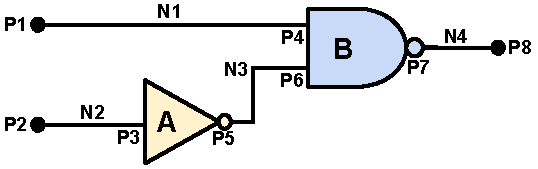
\includegraphics[width=0.7\linewidth]{img/tecnica/circuitExample}
    % \caption{Combinational circuit portion with two logic gates (A and B), four nets (N1 to N4), and eight pins (P1 to P8).}
    \caption[Fragmento de um circuito combinacional]{Fragmento de um circuito combinacional composto por duas portas lógicas (A e B), quatro nets (N1 a N4) e oito pinos (P1 a P8).}
    \label{fig:circuito_exemplo}
\end{figure}

Um estimador de comprimento de interconexão deve ter acesso à informação de quais pinos pertencem a cada Net, bem como às posições dos pinos dentro do leiaute do circuito.
A Figura~\ref{fig:classHierarchyOOD} ilustra uma possível decomposição para o problema de estimativa de comprimento de interconexão seguindo o modelo de programação \ac{ood}.
Este diagrama é composto por dois módulos: \textit{Netlist} e \textit{Placemment}.
O módulo \textit{Netlist} possui duas classes, \textit{Net} e \textit{Pin}, para descrever as interconexões do circuito e os pinos associados.
Para a classe \textit{Pin}, este módulo caracteriza apenas o nome do pino e a rede a que ele pertence, sem qualquer informação de posicionamento.
O módulo \textit{Placemment}, por sua vez, descreve as posições dos pinos.
A seta entre as classes \textit{Pin} e \textit{Net} representam uma relação de agregação, o que significa que a interconeção possui uma referência aos seus pinos, enquanto um pino tem uma referência à sua interconeção proprietária.
A seta entre as duas classes \textit{Pin} representa um relacionamento hierárquico, o que significa que a classe \textit{Pin} do módulo \textit{Placement} estende os atributos do pino do módulo \textit{Netlist}.

\begin{figure}[ht]
    \centering
    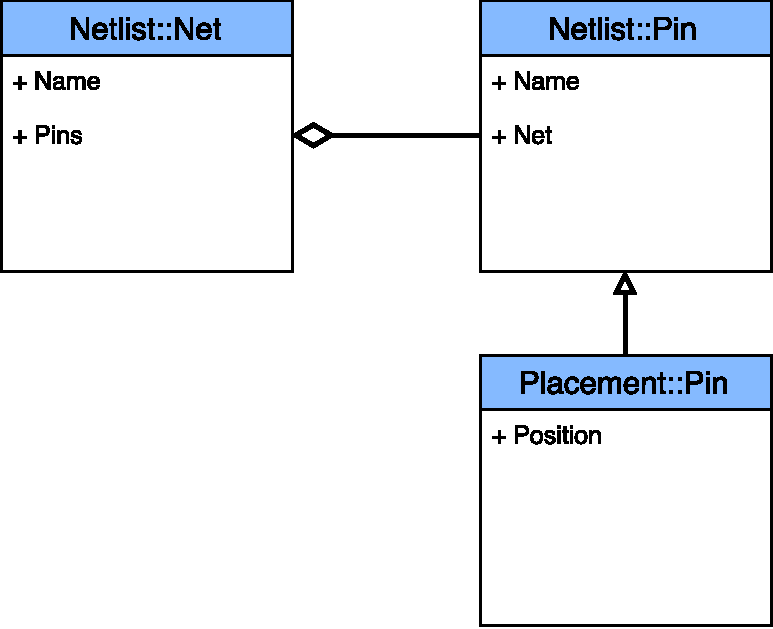
\includegraphics[width=0.5\linewidth]{img/tecnica/classHierarchyOOD}
    % \caption{Class diagram to model wirelength estimation problem with \ac{ood} approach.}
    \caption[Diagrama de classe com OOD]{Diagrama de classe para modelagem da estimativa do comprimento de uma intercenexão seguindo o modelo de programação \ac{ood}}
    \label{fig:classHierarchyOOD}
\end{figure}

Embora possa ser fácil decompor um problema usando o modelo \ac{ood}, a implementação de um software, baseando-se apenas neste modelo de programação, pode levar a uma hierarquia de classes excessivamente complexa.
Esta questão é particularmente crítica no desenvolvimento de uma biblioteca de software, pois é difícil prever, durante o design da biblioteca, como ela será realmente utilizada.
Por exemplo, suponha que outro problema requer informações temporais sobre os pinos do circuito da Figura~\ref{fig:circuito_exemplo}.
Seguindo o modelo de programação \ac{ood}, essas informações temporais podem ser adicionadas naturalmente criando um novo módulo chamado \textit{Timing} e uma nova classe \textit{Pin} (com atributos de temporização dos pinos) neste módulo.
Por sua vez, esta nova classe deve também estender a classe \textit{Pin} do módulo \textit{Netlist}.
Esta nova decomposição resulta na hierarquia de classes mostrada na Figura~\ref{fig:classHierarchyTimingOOD}.

\begin{figure}[ht]
    \centering
    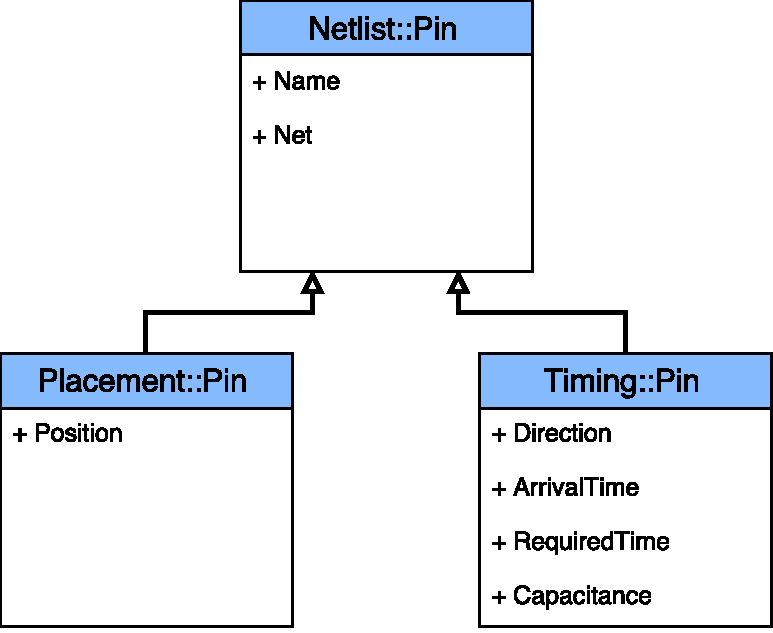
\includegraphics[width=0.5\linewidth]{img/tecnica/classHierarchyTimingOOD}
    % \caption{Class diagram to model when pin timing information is added.}
    \caption[Diagrama de classe de um pino]{Diagrama de classe de um pino com informações de posicionamento e temporais.}
    \label{fig:classHierarchyTimingOOD}
\end{figure}


Agora, suponha que outro desenvolvedor queira usar nossa biblioteca de Physical Design para implementar um algoritmo de \ac{itdp}.
Para fazer isso, este desenvolvedor irá precisar de uma nova classe \textit{Pin} com as informações de posicionamento e temporização.
Em \ac{ood}, isso pode ser realizado através de herança múltipla, onde esta nova classe \textit{Pin} estende as classes \textit{Pin} de \textit{Placemment} e \textit{Timing}.
No entanto, a herança múltipla não é suportada por todas as linguagens de programação, e mesmo quando suportada, não é recomendável porque pode levar a problemas de design~\cite{nystrom2014game}.

Sem recorrer a herança múltipla, a solução consiste em criar uma nova classe \textit{Pin} que se estende do módulo \textit{Placement} ou \textit{Timing}, e repita o código da outra classe (que não foi estendida).
Esta solução está apresentada na Figura~\ref{fig:classITDP}(a) e~\ref{fig:classITDP}(b).
De qualquer forma, não existe uma maneira simples de reutilizar informações de posicionamento e tempo sem ocorrer replicação de código.
A única opção restante é reunir todas as informações na classe \textit{Pin} do módulo \textit{Timing}, fazendo o mesmo estender o do módulo \textit{Placement}.
Esta solução está ilustrada na Figura~\ref{fig:classITDP}(c).
No entanto, nem sempre é necessário ter informações de posicionamento no módulo \textit{Timing}.
Por exemplo, uma ferramenta analize de timing estática pode não precisar de informações de posicionamento durante etapas iniciais do projeto.
Portanto, a adoção da última solução (Figura~\ref{fig:classITDP}(c)) levaria ao desperdício de memória, uma vez que informações desnecessárias seriam armazenadas.

\begin{figure}[!ht]
    \centering
    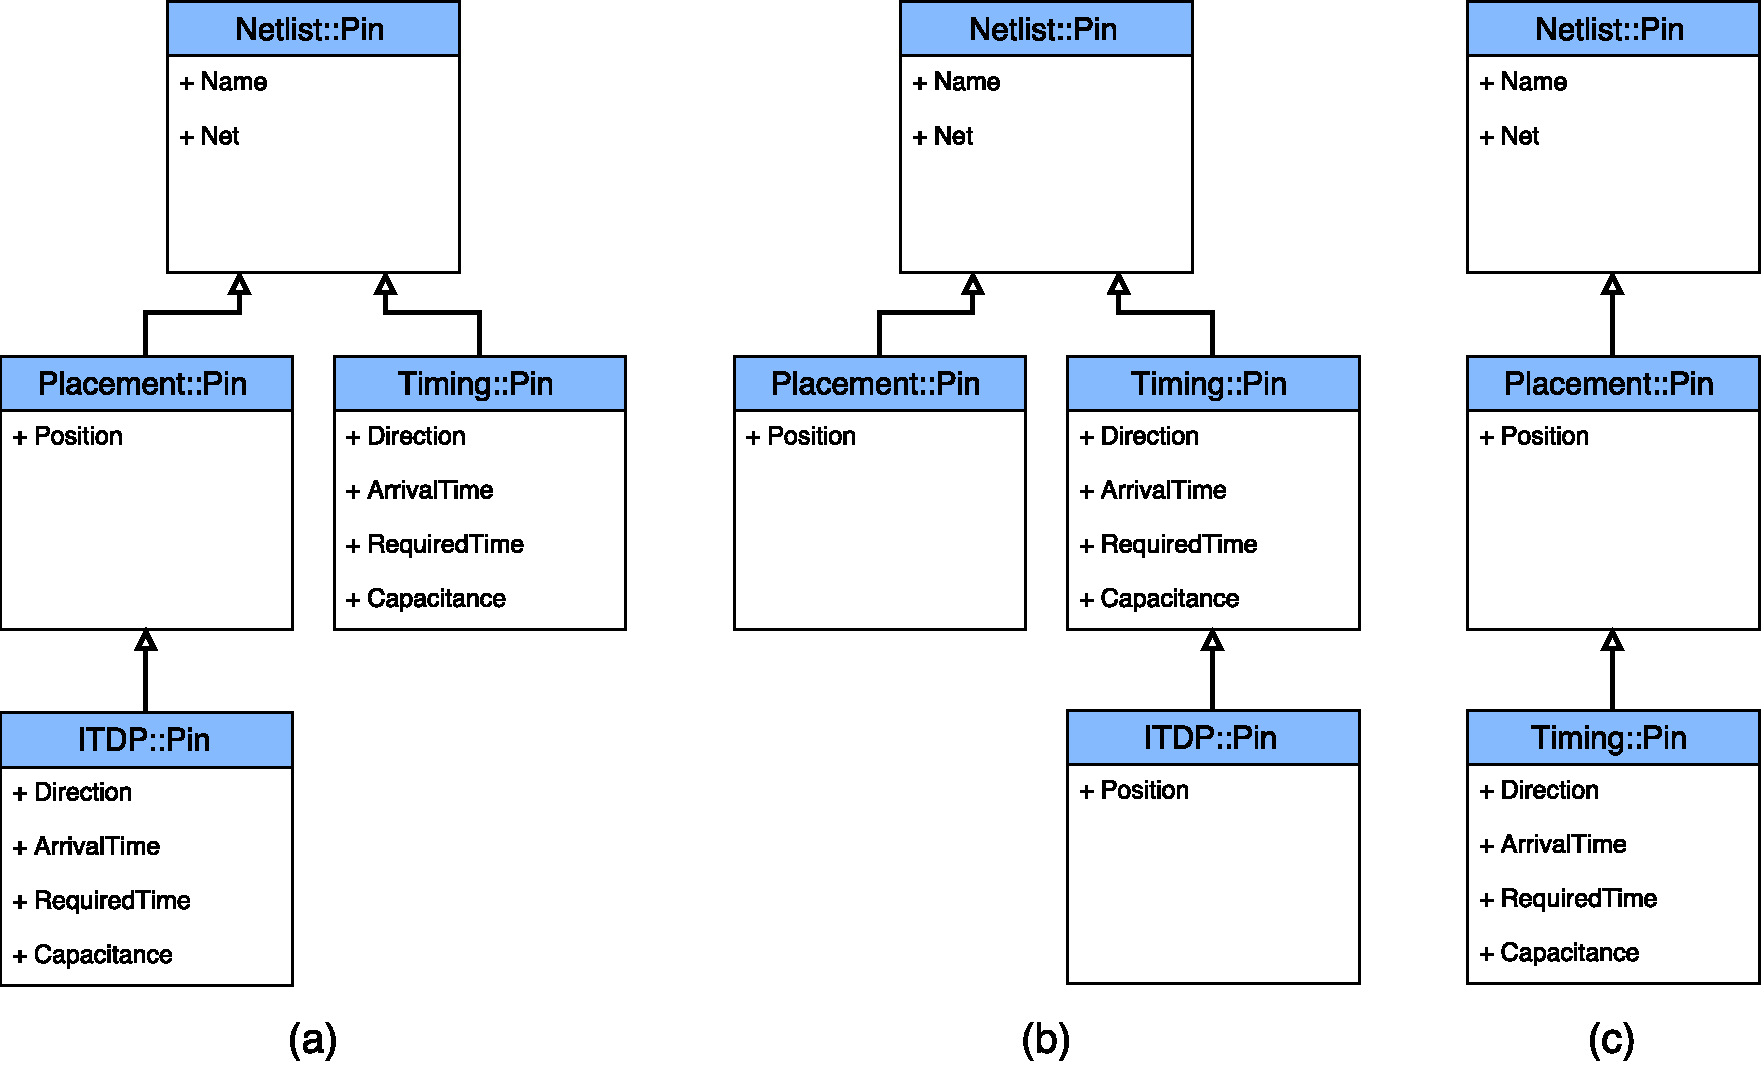
\includegraphics[width=\textwidth]{img/tecnica/ITDPsolutionOOD}
    % \caption{Possible class hierarchy to support information of \textit{Timing} and \textit{Placement} for a timing-driven placement algorithm following \ac{ood} approach.}
    \caption[Hierarquia de classes para suportar \textit{Timing} e \textit{Placement}]{Possível hierarquia de classes para suporte  informações de \textit{Timing} e \textit{Placement} para um algorítmo de \ac{itdp} seguindo o modelo de programação \ac{ood}.}
    \label{fig:classITDP}
\end{figure}

\section{Modelo de Programação Orientado a Dados}
\label{sec:modelo_orientado_dados}

\section{Modelagem dos Dados para Physical Design}
\label{sec:modelagem_physical_design}

\subsection{Estudo de Caso A\@: Verificação dos Limites do Chip}
\label{subsec:problema_A}

\subsection{Estudo de Caso B\@: Estimativa de Interconexão}
\label{subsec:problema_B}

\subsection{Estudo de Caso C\@: Clusterização de Registradores}
\label{subsec:problema_C}


% apresentar modelo de memoria
% apresentar como cache miss funciona
% apresentar ood
% apresentar limitação do ood
% apresentar dod
% apresentar entity system
% Discutir como o DOD reduz o numero de cache misses
% como aplicar o dod em problemas
%     Problema A - limites do chip
%         como seria modelado OOD
%         como seria modelado DOD
%     Problema B - interconexão
%         como seria modelado OOD
%         como seria modelado DOD
%     Problema C - cluster
%         como seria modelado OOD
%         como seria modelado DOD
